\section{Đề ôn thi giữa kỳ 2 toán 10}
\subsection{Phần trắc nghiệm}
Câu trắc nghiệm nhiều phương án lựa chọn. Học sinh trả lời từ
câu 1 đến câu 12. Mỗi câu hỏi học sinh \textit{chỉ chọn một} phương án.

\Opensolutionfile{ans}[Ans/Dapan]
 
\hienthiloigiaiex
\begin{ex}%[0D7N1-1]%[Dự án đề kiểm tra toán khối 10 GHKII NH23-24-Dot2-Đoàn Huy]%[Đề số 2 - CTST]
	Điều kiện để tam thức bậc hai $a x^2+b x+c(a \neq 0)$ nhận giá trị âm với mọi $x \in \mathbb{R}$ là
	\choice
	{$\Delta>0$
	}{$\Delta<0$
	}{$\Delta<0$ và $a>0$
	}{\True $\Delta<0$ và $a<0$}
	\loigiai{
		Áp dụng định lí dấu tam thức bậc hai, ta có kết quả $\Delta<0$ và $a<0$.	
	}
\end{ex}
\begin{ex}%[0D7H1-1]
	Bảng xét dấu sau đây là của tam thức bậc hai nào?
	
	\begin{center}
		
\begin{tikzpicture}
			\tkzTabInit%[nocadre,lgt=1.2,espcl=2]
			{$x$/0.7,$f(x)$/0.7}{$-\infty$,$-2$,$3$,$+\infty$}
			\tkzTabLine{,+,0,-,0,+,}	 
		\end{tikzpicture}
	\end{center}
	
	\choice
	{$x^2-x+6$
	}{$x^2+x+6$
	}{\True $x^2-x-6$
	}{$-x^2+x-6$}
	\loigiai{
		Dựa vào bảng xét dấu ta thấy, $f(x)=0$ có hai nghiệm là $x_1=-2$ và $x_2=3$, dấu của $f(x)$ khi $-2<x<3$ là dấu âm nên chỉ có  $f(x)=x^2-x-6$ thỏa mãn.
	}
\end{ex}
\begin{ex}%[0D7N2-1]
	Nghiệm của bất phương trình $x^2-8x+15 \leq 0$
	\choice
	{\True $x \in \left[3;5\right]$}
	{$x \in \left(3;5\right)$}
	{$x \in \left(-\infty;3\right] \cup \left[5;+\infty\right)$}
	{$x \in \left(-\infty;3\right) \cup \left(5;+\infty\right)$}
	\loigiai{
		Ta có $x^2-8x+15 \leq 0 \Leftrightarrow (x-3)(x-5)\leq 0$ suy ra bảng xét dấu dưới đây
		\begin{center}
			
\begin{tikzpicture}
				\tkzTabInit%[nocadre,lgt=1.2,espcl=2]
				{$x$/0.7,$f(x)$/0.7}{$-\infty$,$3$,$5$,$+\infty$}
				\tkzTabLine{,-,0,+,0,-,}	 
			\end{tikzpicture}
		\end{center}
		Dựa vào bảng xét dấu dễ dàng suy ra được kết quả là $x \in \left[3;5\right]$.
	}
\end{ex}
\begin{ex}%[0D7V1-5]
	Một đường hầm xuyên thẳng qua núi và có mặt cắt là một parabol (thông số như hình bên). Giả sử một chiếc xe tải có chiều ngang $6m$ đi vào vị trí chính giữa miệng hầm. Hỏi chiều cao $h$ của xe tải cần thỏa mãn điều kiện gì để có thể đi vào cửa hầm mà không chạm tường?
	
	\begin{center}
		\begin{tikzpicture}[scale=0.5,>=stealth, font=\footnotesize, line join=round, line cap=round]  
			%\draw[->] (-5,0)--(5,0)node[below]{$x$};
			%\draw[->] (0,-6)--(0,3)node[left]{$y$};
			\draw[samples=100,domain=-6:6] plot (\x,{8-(2/9)*(\x)^2});
			\draw(0,0)node[below left]{$12m$};
			\draw(0,4)node[below left]{$8m$};
			\foreach \x in {-6,-5.5,-5,-4.5,-4,-3.5,-3,-2.5,-2,-1.5,-1,-0.5,0,0.5,1,1.5,2,2.5,3,3.5,4,4.5,5,5.5,6}{
				\draw (\x,0) circle (1pt);
			}	
			\foreach \x in {0.5,1,1.5,2,2.5,3,3.5,4,4.5,5,5.5,6,6.5,7,7.5,8}{
				\draw (0,\x) circle (1pt);
			}		
		\end{tikzpicture}
	\end{center}
	
	\choice
	{\True $0<h<6$
	}{$0<h \leq 6$
	}{$0<h<7$
	}{$0<h \leq 7$}
	\loigiai{
		Chọn hệ trục tọa độ như hình bên dưới.
		\begin{center}
			\begin{tikzpicture}[scale=0.5,>=stealth, font=\footnotesize, line join=round, line cap=round]  
				\draw[->] (0,0)--(13,0)node[below]{$x$};
				\draw[->] (0,0)--(0,13)node[left]{$y$};
				\draw[samples=100,domain=0:12,red] plot (\x,{(8/3)*(\x)-(2/9)*(\x)^2});
				\foreach \x in {0,2,3,4,6,8,9,10,12}{
					\draw (\x,0) node[below]{$ \x $} circle (1pt);
				}	
				\foreach \x in {5,6,8,10}{
					\draw (0,\x) node[left]{$ \x $} circle (1pt);
				}
				%	\foreach \x in {1,2,3,4,5,6,7,8}{
					%\draw (6,\x) circle (1pt);				}	
				\draw[dashed] (0,8)--(6,8)--(6,0);
				\draw[dashed] (3,0)--(3,6);
				\draw[dashed] (9,0)--(9,6)--(3,6);
				\draw (3,6) node[left]{A} circle (1pt);
				\draw (9,6) node[right]{B} circle (1pt);
			\end{tikzpicture}
		\end{center}
		Parabol có phương trình dạng $y=ax^2+bx$. Theo đề bài ra ta có parabol đi qua các điểm $(12;0)$ và $(6;8)$. Suy ra $\heva{& 144a+12b=0\\& 36a+6b=8} \Leftrightarrow \heva{& a=-\dfrac{2}{9}\\&b=\dfrac{8}{3}.}$\\
		Do đó $y=-\dfrac{2}{9}x^2+\dfrac{8}{3}x$. Do chiếc xe tải có chiều ngang $6m$ đi vào vị trí chính giữa hầm nên xe sẽ chạm vào tường tại điểm $A(3;6)$ và điểm $B(9;6)$. Khi đó chiều cao của xe là $6m$. Vậy điều kiện để xe tải có thể đi vào hàm mà không chạm tường là $0<h<6$.
	}
\end{ex}
\begin{ex}%[0D7H3-2]
	Tập nghiệm của phương trình $\sqrt{x^2-4x+3}=x+1$ là
	\choice
	{$S=\varnothing$
	}{\True $S=\left\{\dfrac{1}{3}\right\}$
	}{$S=\{3\}$
	}{$S=\{1\}$}
	\loigiai{
		\noindent Ta có $\sqrt{x^2-4x+3}=x+1 \Leftrightarrow \heva{&x+1 \geq 0 \\ & x^2-4x+3 = (x+1)^2} \Leftrightarrow \heva{&x \geq -1 \\ & -6x+2 = 0.}$\\
		Phương trình $-6x+2 = 0$ có nghiệm $x=\dfrac{1}{3}$. Ta thấy $x=\dfrac{1}{3}$ thoản mãn $x \geq -1$.\\
		Vậy tập nghiệm của phương trình là $S=\left\{\dfrac{1}{3}\right\}$.
	}
\end{ex}
\begin{ex}%[0D7H3-1]
	Số nghiệm của phương trình $\sqrt{x^2-3x+2}=\sqrt{2 x^2-7|x|+4}$ là
	\choice
	{$1$
	}{$2$
	}{$3$
	}{\True $4$}
	\loigiai{
		\noindent Ta có $\sqrt{x^2-3x+2}=\sqrt{2 x^2-7|x|+4}$\\ $ \Leftrightarrow \heva{& \hoac{&x \geq 2 \\ & x \le 1} \\ & \hoac{&|x| \geq \frac{7+\sqrt{17}}{4} \\ & 0 \le |x| \le \frac{7-\sqrt{17}}{4}.}}$
		$\Leftrightarrow \hoac{& x \geq \frac{7+\sqrt{17}}{4} \\& -\frac{7-\sqrt{17}}{4} \le x \le \frac{7-\sqrt{17}}{4} \\& x \le -\frac{7+\sqrt{17}}{4}.}$\\
		Bình phương hai vế ta có $x^2-3x+2 = 2 x^2-7|x|+4$.\\
		\noindent Xét $x \geq 0 \Leftrightarrow x^2 -4x+2=0$. Phương trình có hai nghiệm thỏa mãn, $x_1=2+\sqrt{2}$ và $x_2=2-\sqrt{2}$.\\
		\noindent Xét $x \le 0 \Leftrightarrow x^2 +10x+2=0$. Phương trình có hai nghiệm thỏa mãn, $x_3=-5+\sqrt{23}$ và $x_4=-5-\sqrt{23}$.\\
		Vậy phương trình có $4$ nghiệm.
		
		
	}
\end{ex}
\begin{ex}%[0H9N1-3]
	Trong mặt phẳng toạ độ $Oxy$ cho các véc-tơ $\vec{a}, \vec{b}, \vec{c}, \vec{d}$ được vẽ ở hình bên dưới. Ta có các khẳng định sau
	
	\begin{center}
		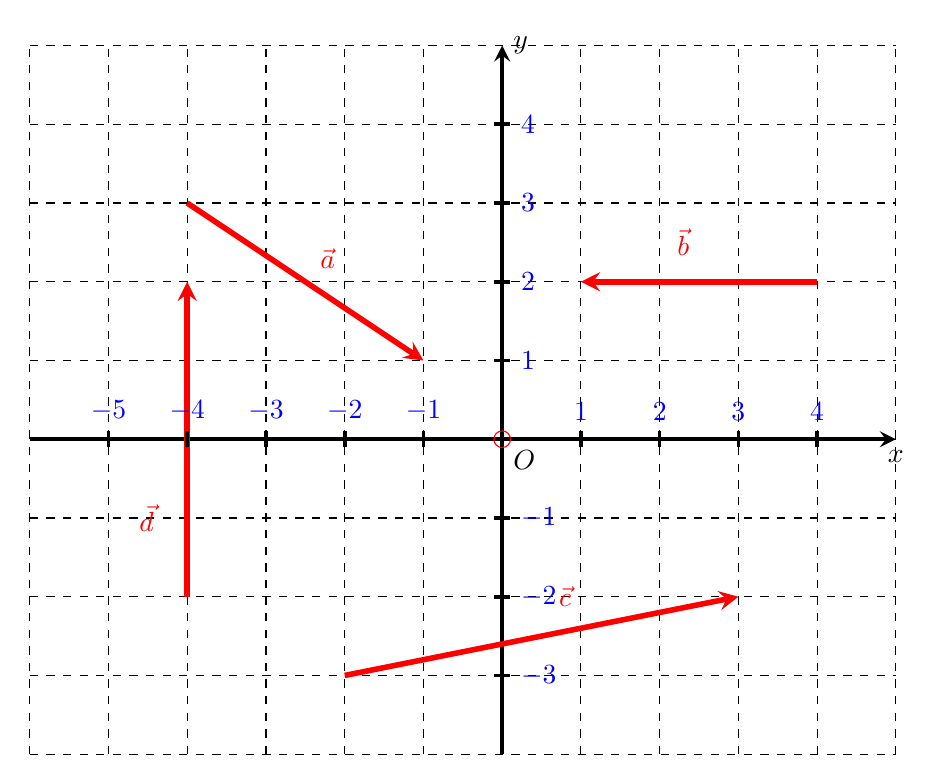
\begin{tikzpicture}[>=stealth,x=1cm,y=1cm]
			\draw[dashed] (-6,-4) grid (5,5);
			\draw[->,line width = 1.5pt,black] (-6,0)--(0,0)%
			node[below right]{$O$}--(5,0) node[below]{$x$};
			\draw[->,line width = 1.5pt,black] (0,-4) --(0,5) node[right]{$y$};
			\draw[->,line width = 2pt,red] (-4,3) --(-1,1);
			\draw[fill=none,red] (-2,2.3) node[left]{$\vec{a}$};
			\draw[->,line width = 2pt,red] (4,2) --(1,2);
			\draw[fill=none,red] (2.5,2.5) node[left]{$\vec{b}$};
			\draw[->,line width = 2pt,red] (-2,-3) --(3,-2);
			\draw[fill=none,red] (1,-2) node[left]{$\vec{c}$};
			\draw[->,line width = 2pt,red] (-4,-2) --(-4,2);
			\draw[fill=none,red] (-4.3,-1) node[left]{$\vec{d}$};
			4	\foreach \x in {-5,-4,-3,-2,-1,1,2,3,4}{
				\draw[-,line width=1.3pt] (\x,-.1)--(\x,.1) node[above,blue]{$\x$};%Oy
			}
			\foreach \y in {-3,-2,-1,1,2,3,4}{
				\draw[-,line width=1.3pt] (-.1,\y)--(.1,\y) node[right,blue]{$\y$};%Oy
			}
			\draw[fill=none,red] (0,0) circle(3pt);
		\end{tikzpicture}
	\end{center}
	
	\noindent \textbf{A.}$\vec{a}=(2;-3)$. \hspace*{2cm} \textbf{B.}$\vec{b}=(-3;0)$.\hspace*{2cm} \textbf{C.}$\vec{c}=(5;1)$.\hspace*{2cm} \textbf{D.}$\vec{d}=(4;0)$.\\
	\noindent Số khẳng định đúng là
	\choice
	{$0$
	}{$1$
	}{\True $2$
	}{$3$}
	\loigiai{
		\noindent Để biết được tọa độ một véc-tơ ta tịnh tiến véc-tơ đó sao cho gốc tọa độ trùng với điểm đầu của véc-tơ. Khi đó tọa độ điểm cuối của véc-tơ chính là tọa độ của véc-tơ. Áp dụng với các véc-tơ, ta có
		$\vec{a}=(3;-2), \vec{b}=(-3;0)$ $\vec{c}=(5;1), \vec{d}=(0;4)$.\\
		Vậy ta có số khẳng định đúng là $2$.
	}
\end{ex}
\begin{ex}%[0H9N1-2]
	Trong mặt phẳng tọa độ $Oxy$, cho $\vec{a}=(2;-3), \vec{b}=(-2;5)$. Toạ độ của véc-tơ $-\vec{a}+3\vec{b}$ là
	\choice
	{$(8;18)$
	}{$(-8;-18)$
	}{\True $(-8;18)$
	}{$(8 ;-18)$}
	\loigiai{
		\noindent Toạ độ của véc-tơ $-\vec{a}+3\vec{b} = -(2;-3)+3(-2;5)= (-2;3)+(-6;15)=(-8;18)$.
	}
\end{ex}
\begin{ex}%[0H9H3-2]
	Trong mặt phẳng tọa độ $Oxy$, cho hai điểm $A(5;4), B(-1;0)$. Đường trung trực của đoạn thẳng $AB$ có phương trình là
	\choice
	{$x-2y+5=0$
	}{\True $3x+2y-10=0$
	}{$3x+2y-5=0$
	}{$2x+3y-1=0$}
	\loigiai{
		\noindent Phương trình đường trung trực của đoạn thẳng $AB$ là đường thẳng đi qua trung điểm $I$ của $AB$ và nhận $\overrightarrow{AB}$ làm véc-tơ pháp tuyến.\\
		Tọa độ $I = (\dfrac{5-1}{2}; \dfrac{4+0}{2}) =(2;2)$, $\overrightarrow{AB} =(-6;-4)$.\\
		\noindent Vậy phương trình đường thẳng là $-6(x-2)-4(y-2)=0 \ \Leftrightarrow -6x-4y +20 \Leftrightarrow 3x+2y-10=0$.
	}
\end{ex}
\begin{ex}%[0H9H3-2]
	Trong mặt phẳng toạ độ $Oxy$, cho ba điểm $A(5;2), B(5;-2), C(4;-3)$. Đường thẳng đi qua điểm $A$ và vuông góc với đường thẳng $BC$ có phương trình là
	\choice
	{$x-y+7=0$
	}{\True $x+y-7=0$
	}{$x-y-5=0$
	}{$x+y=0$}
	\loigiai{
		\noindent Phương trình đường thẳng đi qua $A$  và vuông góc với $BC$ là đường thẳng đi qua $A$  nhận $\overrightarrow{BC}$ làm véc-tơ pháp tuyến, $\overrightarrow{BC} =(-1;-1)$.\\
		\noindent Vậy phương trình đường thẳng là $-1(x-5)-1(y-2)=0 \ \Leftrightarrow -x-y +7 \Leftrightarrow x+y-7=0$.
	}
\end{ex}
\begin{ex}%[0H9H4-1]
	Phương trình đường tròn có tâm $I(1;2)$ và đi qua điểm $A(-1;3)$ là
	\choice
	{$(x+1)^2+(y+2)^2=25$
	}{$(x+1)^2+(y+2)^2=5$
	}{\True $(x-1)^2+(y-2)^2=5$
	}{$(x-1)^2+(y-2)^2=25$}
	\loigiai{
		\noindent Khi đường tròn cho ở dạng $(x-a)^2+(y-b)^2=R^2$ thì đường tròn có tâm tâm $I(a ; b)$ và bán kính $R$.\\
		\noindent Áp dụng với các trường hợp cụ thể trên ta có tâm $I(1;2)$ và đi qua điểm $A(-1;3)$ sẽ có bán kính $R=IA$. Ta có $R^2= (-1-1)^2+(3-2)^2=5$.\\
		\noindent Vậy phương trình đường tròn đi qua điểm $A$ có tâm $I$ là $(x-1)^2+(y-2)^2=5$.
	}
\end{ex}
\begin{ex}%[0H9H4-1]
	Trong mặt phẳng toạ độ $Oxy$, cho hai điểm $A(-4;6), B(-2;4)$. Phương trình đường tròn có đường kính $AB$ là
	\choice
	{\True $(x+3)^2+(y-5)^2=2$
	}{$(x+3)^2+(y+5)^2=2$
	}{$(x-3)^2+(y+5)^2=2\sqrt{2}$
	}{$(x-3)^2+(y-5)^2=2\sqrt{2}$}
	\loigiai{
		\noindent Đường tròn có đường kính $AB$ sẽ có tâm $I$ là trung điểm của $AB$ và bán kính $R=\dfrac{AB}{2}$.\\
		\noindent Áp dụng với trường hợp $A(-4;6)$ và $B(-2;4)$ ta có $I(-3;1)$ và bán kính $R=\dfrac{\sqrt{(-2-(-4))^2 +(4-6)^2}}{2} = \sqrt{2}$.\\
		\noindent Vậy phương trình đường tròn cần tìm là $(x+3)^2+(y-5)^2=2$.
	}
\end{ex}

  
\Closesolutionfile{ans}
\bangdapan{Dapan}
\subsection{Câu trắc nghiệm đúng sai}
Học sinh trả lời từ câu 1 đến câu 4.
Trong mỗi ý \circlenum{A}, \circlenum{B}, \circlenum{C} và \circlenum{D} ở mỗi câu, học sinh chọn đúng hoặc sai.
\setcounter{ex}{0}
\LGexTF
\Opensolutionfile{ansbook}[ansbook/DapanDS]
\Opensolutionfile{ans}[Ans/DapanT]
\hienthiloigiaiex
\begin{ex}%[0D3H2-3]%[Dự án đề kiểm tra Toán K10 GHKII NH2023-24-Dot 1- DoanHuy]%[Deso2-CTST]
	Dựa vào đồ thị hàm số bậc hai $y=f(x)$ và $y=g(x)$ được cho trong mỗi hình sau. Khi đó:
	\begin{center}
		\begin{table}[!htp]
		\begin{tabular}{|c|c|}
			\hline			
			\begin{tikzpicture}[scale=0.5,>=stealth, font=\footnotesize, line join=round, line cap=round]  
				\draw[->] (-5,0)--(5,0)node[below]{$x$};
				\draw[->] (0,-6)--(0,3)node[left]{$y$};
				\draw[samples=100,domain=-2.5:2.5] plot (\x,{(\x)^2-4});
				\draw(0,0)node[below left]{$O$};
				\foreach \x in {-5,-4,-3,-2,-1,1,2,3,4}{
					\draw (\x,0) node[below]{$\x$} circle (1pt);
				}	
				\foreach \x in {-5,-4,-3,-2,-1,1,2}{
					\draw (0,\x) node[left]{$\x$} circle (1pt);
				}		
			\end{tikzpicture}	&  \begin{tikzpicture}[scale=0.5,>=stealth, font=\footnotesize, line join=round, line cap=round]  
				\draw[->] (-3,0)--(8,0)node[below left]{$x$};
				\draw[->] (0,-6)--(0,3)node[left]{$y$};
				\draw[samples=100,domain=1:6] plot (\x,{-(\x)^2+7*(\x)-12});
				\draw(0,0)node[above left]{$O$};
				\foreach \x in {-2,-1,1,2,3,4,5,6,7}{
					\draw (\x,0) node[below]{$\x$} circle (1pt);			
				}
				\foreach \x in {-5,-4,-3,-2,-1,1,2}{
					\draw (0,\x) node[left]{$\x$} circle (1pt);
				}
			\end{tikzpicture}
			\\
			\hline
			$y=f(x)$	&  $y=g(x)$ \\
			\hline
		\end{tabular}		
	\end{table}
	\end{center}
	\choiceTF
	{\True Đồ thị hàm số $y=f(x)$ cắt trục hoành tại hai điểm $(-2;0)$ và $(2;0)$}
	{\True Đồ thị hàm số $y=g(x)$ cắt trục hoành tại hai điểm $(3;0)$ và $(4;0)$}
	{Tam thức bậc hai $f(x)$ có bảng xét dấu
		\begin{center}
			
\begin{tikzpicture}
				\tkzTabInit%[nocadre,lgt=1.2,espcl=2]
				{$x$/0.7,$f(x)$/0.7}{$-\infty$,$3$,$4$,$+\infty$}
				\tkzTabLine{,-,0,+,0,-,}	 
			\end{tikzpicture}
		\end{center}
	}
	{Tam thức bậc hai $g(x)$ có bảng xét dấu
		\begin{center}
			
\begin{tikzpicture}
				\tkzTabInit%[nocadre,lgt=1.2,espcl=2]
				{$x$/0.7,$g(x)$/0.7}{$-\infty$,$-2$,$2$,$+\infty$}
				\tkzTabLine{,+,0,-,0,+,}	 
			\end{tikzpicture}
		\end{center}
	}
	\loigiai{	
		\begin{itemize}
			\item Đồ thị hàm số $y=f(x)$ cắt trục hoành tại hai điểm $(-2;0)$ và $(2;0)$ nên tam thức bậc hai $f(x)$ có hai nghiệm là $x_1=-2$, $x_2=2$. Đồ thị có bề lõm quay lên trên nên hệ số $a > 0$. Do đó, ta có bảng xét dấu: \\
			\begin{center}
				
\begin{tikzpicture}
					\tkzTabInit%[nocadre,lgt=1.2,espcl=2]
					{$x$/0.7,$f(x)$/0.7}{$-\infty$,$-2$,$2$,$+\infty$}
					\tkzTabLine{,+,0,-,0,+,}	 
				\end{tikzpicture}
			\end{center}
			\item Đồ thị hàm số $y=g(x)$ cắt trục hoành tại hai điểm $(3;0)$ và $(4;0)$ nên tam thức bậc hai $g(x)$ có hai nghiệm là $x_1=3$, $x_2=4$. Đồ thị có bề lõm quay lên xuống nên hệ số $a < 0$. Do đó, ta có bảng xét dấu: \\
			\begin{center}
				
\begin{tikzpicture}
					\tkzTabInit%[nocadre,lgt=1.2,espcl=2]
					{$x$/0.7,$g(x)$/0.7}{$-\infty$,$3$,$4$,$+\infty$}
					\tkzTabLine{,-,0,+,0,-,}	 
				\end{tikzpicture}
			\end{center}
		\end{itemize}
	}
\end{ex}
\begin{ex}%[0D7H3-2]%[Dự án đề kiểm tra Toán K10 GHKII NH2023-24-Dot 1- DoanHuy]%[Deso2-CTST]
	Cho phương trình $\sqrt{2 x^2+x-6}=x+2\left({ }^*\right)$ Khi đó
	\choiceTF
	{\True Bình phương 2 vế phương trình ta được $x^2-3 x-10=0$
	}{ Điều kiện của phương trình $\left(^*\right)$ là $x \geq 2$
	}{\True Phương trình (*) có 2 nghiệm
	}{\True Tổng bình phương các nghiệm của phương trình (*) bằng $20$}
	\loigiai{
		\noindent Ta có $\sqrt{2x^2+x-6}=x+2 \Leftrightarrow \heva{&x+2 \geq 0 \\ & 2x^2+x-6 = (x+2)^2} \Leftrightarrow \heva{&x \geq -2 \\ & x^2-3x-10 = 0.}$\\
		Phương trình $x^2-3x-10=0$ có hai nghiệm $x_1=-2,x_2=5$. Ta thấy $x_1=-2$ và $x_2=5$ đều thoản mãn $x \geq -2$.\\
		Vậy tập nghiệm của phương trình là $S=\{-2;5\}$.
	}
\end{ex}
\begin{ex}%[0H9H3-2]%[Dự án đề kiểm tra Toán K10 GHKII NH2023-24-Dot 1- DoanHuy]%[Deso2-CTST]
	Trong mặt phẳng tọa độ $O x y$, cho tam giác $D E F$ có $D(1 ;-1), E(2 ; 1), F(3 ; 5)$. Khi đó
	\choiceTF
	{Đường thẳng vuông góc với đường thẳng $EF$ nhận $\overrightarrow{EF}$ là một véc-tơ chỉ phương
	}{Phương trình đường cao kẻ từ $D$ là $x+y=0$
	}{\True Gọi $I$ là trung điểm của $DF$. Tọa độ của điểm $I$ là $(2;2)$
	}{\True Đường trung tuyến kẻ từ $E$ có phương trình là $x-2=0$}
	\loigiai{
		\noindent Đường cao kẻ từ $D$ là đường thẳng vuông góc với đường thẳng $EF$ nên nhận $\overrightarrow{EF}(1;4)$ là véc-tơ pháp tuyến. Do đó, đường cao kẻ từ $D$ có phương trình là 
		$(x-1)+4(y+1)=0 \Leftrightarrow x+4y+3=0$.\\
		Gọi $I$ là trung điểm của $DF$. Tọa độ của điểm $I$ là $(2;2)$. Đường trung tuyến kẻ từ $E$ có véc-tơ chỉ phương là $\overrightarrow{EI}(0;1)$ nên nhận $\overrightarrow{n}(1;0)$ là một véc-tơ pháp tuyến. Do đó, đường trung tuyến kẻ từ $E$ có phương trình là $x-2=0$.
	}
\end{ex}
\begin{ex}%[0H9H4-1]%[Dự án đề kiểm tra Toán K10 GHKII NH2023-24-Dot 1- DoanHuy]%[Deso2-CTST]
	Xác định tính đúng, sai của các khẳng định sau:
	\choiceTF
	{\True Cho $(C):(x+3)^2+(y-2)^2=4$, khi đó $(C)$ có tâm $I(-3;2)$ và bán kính $R=2$
	}{\True Cho $(C): x^2+y^2=1$, khi đó $(C)$ có tâm $O(0;0)$ và bán kính $R=1$
	}{Cho $(C): x^2+y^2-6 x+2 y-6=0$, khi đó $(C)$ có tâm $I(3;-1)$ và bán kính $R=3$
	}{Cho $(C): x^2+y^2-4x-5=0$, khi đó $(C)$ có tâm $I(2;0)$ và bán kính $R=2$
	}
	\loigiai{
		\noindent Khi đường tròn cho ở dạng $(x-a)^2+(y-b)^2=R^2$ thì đường tròn có tâm tâm $I(a ; b)$ và bán kính $R$.\\
		\noindent Khi đường tròn cho ở dạng $x^2+y^2-2ax-2by+c=0$ với điều kiện đã được thỏa mãn là $ a^2+b^2-c >0 $ thì đường tròn có tâm tâm $I(a ; b)$ và bán kính $R = \sqrt{a^2+b^2-c}$. \\
		\noindent Áp dụng với các trường hợp cụ thể trên ta có
		\begin{itemize}
			\item Trường hợp $(C):(x+3)^2+(y-2)^2=4$ có tâm $I(-3 ; 2)$ và bán kính $R=2$.
			\item Trường hợp $(C): x^2+y^2=1$ có tâm $O(0 ; 0)$ và bán kính $R=1$.
			\item Trường hợp $(C): x^2+y^2-6x+2y-6=0$. Đặt $a=\dfrac{-6}{-2}=3, b=\dfrac{2}{-2}=-1, c=-6$. Đường tròn $(C)$ có tâm $I(3 ;-1)$ và bán kính $R=\sqrt{a^2+b^2-c}=\sqrt{9+1+6}=4$.
			\item Trường hợp $(C): x^2+y^2-4x-5=0$. Đặt $a=\dfrac{-4}{-2}=2, b=\dfrac{0}{-2}=0, c=-5$. Đường tròn $(C)$ có tâm $I(2 ; 0)$ và bán kính $R=\sqrt{a^2+b^2-c}=\sqrt{4+0+5}=3$.		
		\end{itemize}
	}
\end{ex}


\Closesolutionfile{ans}
\Closesolutionfile{ansbook}

\begin{center}
	\textbf{\textsf{BẢNG ĐÁP ÁN ĐÚNG SAI}}
\end{center}
\input{Ansbook/DapanDS}

\subsection{Phần tự luận}

\hienthiloigiaibt
%%%=============BT_1=============%%%
\begin{bt}%[0D7V1-5]%[Dự án đề kiểm tra toán khối 10 GHKII NH23-24-Dot2-Đỗ Viết Lân]%[Đề số 2 - CTST]
Một vật chuyển động có vận tốc $v$ (mét/giây) được biểu diễn theo thời gian $t$ (giây) bằng công thức $v(t) = \dfrac{1}{2}t^2-4t+10$.
\begin{enumerate}
\item Hỏi sau tối thiểu bao nhiêu giây thì vận tốc của vật không bé hơn $10\,\mathrm{m/s}$?
\item Trong $10$ giây đầu tiên, vận tốc của vật đạt giá trị nhỏ nhất bằng bao nhiêu?
\end{enumerate}
\loigiai{
\begin{enumerate}
\item Để vận tốc của vật không dưới $10\,\mathrm{m/s}$ ta xét bất phương trình $v(t) \geq 10 \Leftrightarrow t^2-8t\geq 0$.\\
Xét $f(t) = t^2 - 8t$; $f(t) = 0 \Leftrightarrow \hoac{&t=0\\&t=8}$. Ta có bảng xét dấu như sau
\begin{center}

\begin{tikzpicture}
\tkzTabInit
{$t$/1,$f(t)$/1}
{$-\infty$,$0$,$8$,$+\infty$}
\tkzTabLine{,+,z,-,z,+,}
\end{tikzpicture}
\end{center}
Ta có $f(t) \geq 0 \Leftrightarrow t \geq 8$ (do $t >0$). Vậy sau tối thiểu $8$ giây, vật sẽ đạt vận tốc $10\,\mathrm{m/s}$.
\item Xét $v(t) = \dfrac{1}{2}t^2-4t+10$ với $-\dfrac{b}{2a} = 4$ và $a>0$. Ta có bảng biến thiên trên đoạn $[0;10]$ như sau
\begin{center}
\begin{tikzpicture}
\tkzTabInit
{$x$/1,$v(t)$/2}
{$0$,$4$,$10$}
\path
	(N11) node[below](1) {${}$}
	(N22) node[above](2){$2$}
	(N31) node[below](3) {${}$}
;
\foreach \x/\y in {1/2,2/3}
	\draw [-stealth] (\x)--(\y);
\end{tikzpicture}
\end{center}
Vậy, ở giây thứ tư thì vật đạt vận tốc nhỏ nhất là $2\,\mathrm{m/s}$.
\end{enumerate}
}
\end{bt}

\begin{bt}%[0D7H3-1]
Tìm nghiệm của phương trình $\sqrt{2x^2+5} = \sqrt{x^2-x+11}$.
\loigiai{
Bình phương hai vế của phương trình ta có 
$$2x^2+5 = x^2-x+11 \Leftrightarrow x^2 + x - 6 = 0 \Leftrightarrow \hoac{&x = 2\\&x=-3}.$$
Thử lại, thay $x = 2$ vào phương trình $\sqrt{13}=\sqrt{13}$ (thỏa mãn).\\
Thay $x=-3$ vào phương trình $\sqrt{23} = \sqrt{23}$ (thỏa mãn).\\
Vậy $S = \{2;-3\}$.
}
\end{bt}

\begin{bt}%[0H9V2-3]
Cho các véc-tơ $\vec{a} = (1;-2)$, $\vec{c} = (m+n;-m-4n)$. Tìm hai số $m$, $n$ sao cho $\vec{c}$ cùng phương với $\vec{a}$ và $|\vec{c}| = 3\sqrt{5}$.
\loigiai{
Ta có $\vec{c}$ cùng phương với $\vec{a}$ nên $\dfrac{m+n}{1} = \dfrac{-m-4n}{-2} \Leftrightarrow m = 2n$. Suy ra $\vec{c} = (3n;-6n)$.\\
Lại có $|\vec{c}| = 3\sqrt{5} \Leftrightarrow \sqrt{(3n)^2+(-6n)^2} = 3\sqrt{5} \Leftrightarrow n = \pm 1$.\\
Vậy $\heva{&m=2\\&n=1}$; $\heva{&m=-2\\&n=-1}$.
}
\end{bt}

\begin{bt}%[0H9C3-2]
Viết phương trình đường thẳng $\Delta$ biết rằng $\Delta$ đi qua điểm $E(2;3)$, đồng thời cắt các tia $Ox$, $Oy$ tại các điểm $M$, $N$ (khác gốc tọa độ $O$) biết rằng $OM+ON$ bé nhất.
\loigiai{
Giả sử $\Delta$ cắt $Ox$ tại $M(m;0)\, (m>0)$ và cắt $Oy$ tại $N(0;n)\, (n>0)$.\\
Ta có phương trình đường thẳng $\Delta$ là $\dfrac{x}{m}+\dfrac{y}{n}=1$.\\
Vì $\Delta$ đi qua điểm $E$ nên $\dfrac{2}{m}+\dfrac{3}{n} = 1$.\\
Suy ra $m = \dfrac{2n}{n-3}$. Do $m>0$ nên $n>3$.\\
Ta có $OM+ON = m+ n = \dfrac{2n}{n-3}+n = 2 + \dfrac{6}{n-3}+n = 5+\dfrac{6}{n-3}+(n-3) \geq 5 + 2\sqrt{6}$.\\
Dấu bằng xảy ra khi và chỉ khi $\dfrac{6}{n-3}=n-3 \Leftrightarrow n = 3+\sqrt{6}$.\\
Suy ra $m=\dfrac{2\left(3+\sqrt{6}\right)}{3+\sqrt{6}-3}=2+\sqrt{6}$. Do đó $\Delta\colon \dfrac{x}{2+\sqrt{6}}+\dfrac{y}{3+\sqrt{6}} -1 = 0$.
}
\end{bt}

\begin{bt}%[0H9V4-1]
Tìm tất cả các giá trị của tham số $m$ để phương trình $x^2+y^2-2(m+1)x+2my+m^2+4=0$ là phương trình đường tròn.
\loigiai{
Ta có $a = m+1$, $b = -m$, $c = m^2+4$.\\
Để phương trình đã cho là phương trình đường tròn thì 
\begin{eqnarray*}
a^2+b^2-c>0 &\Leftrightarrow& (m+1)^2 + (-m)^2-(m^2+4) > 0 \\
&\Leftrightarrow & m^2 + 2m - 3 > 0\\
&\Leftrightarrow & \hoac{&m>1\\&m<-3}.
\end{eqnarray*} 
}
\end{bt}
 